\clearpage
\VerdierPhysicalPageAnchor{0096}%
\begingroup
\setlength{\abovedisplayskip}{3pt plus 2pt minus 2pt}%
\setlength{\belowdisplayskip}{3pt plus 2pt minus 2pt}%
\VerdierSemanticAnchor{ch1-3-3-2-open-morphism-continuation}
此态射在 $\operatorname{comp}(C)$ 中属于态射 $u\colon X\to Y$ 的同伦类。
\VerdierSemanticAnchor{ch1-3-3-2-representative}
于是得到 $\operatorname{Tr}_1(C)$ 的一个对象：
$X\xrightarrow{\dot f}Y$。
\VerdierSemanticAnchor{ch1-3-3-2-completion-cone}
特异三角
\begin{equation*}
  X\xrightarrow{u}Y\xrightarrow{\dot p(f)}c(f)
  \xrightarrow{\dot q(f)}X[1]
\end{equation*}
\VerdierSemanticAnchor{ch1-3-3-2-completion-conclusion}
包含态射 $u$。

\VerdierSemanticAnchor{ch1-3-3-3}
\noindent\textbf{命题 3.3.3. (TRII)}\quad
\VerdierSemanticAnchor{ch1-3-3-3-trii}
\textit{$K(C)$ 的三角
$X\xrightarrow{u}Y\xrightarrow{v}Z\xrightarrow{w}X[1]$ 是特异三角，
当且仅当三角
$Y\xrightarrow{v}Z\xrightarrow{w}X[1]\xrightarrow{-u[1]}Y[1]$
是特异三角。}

\VerdierSemanticAnchor{ch1-3-3-3-proof-forward}
设三角 $X\xrightarrow{u}Y\xrightarrow{v}Z\xrightarrow{w}X[1]$
是特异三角。于是它同构于一个如下形式的三角：

\VerdierSemanticAnchor{ch1-3-3-3-cone-model}
\begin{equation*}
  X'\xrightarrow{\dot f}Y'\xrightarrow{\dot p(f)}c(f)
  \xrightarrow{\dot q(f)}X'[1],
\end{equation*}
其中 $X'\xrightarrow{\dot f}Y'$ 是 $\operatorname{Tr}_1(C)$ 的一个对象。
因此只需证明三角

\VerdierSemanticAnchor{ch1-3-3-3-rotated-model}
\begin{equation*}
  Y'\xrightarrow{\dot p(f)}c(f)\xrightarrow{\dot q(f)}X'[1]
  \xrightarrow{-\dot f[1]}Y'[1],
\end{equation*}
是特异三角。由 (3.2.6)，图

\VerdierSemanticAnchor{ch1-3-3-3-comparison}
\begin{center}
  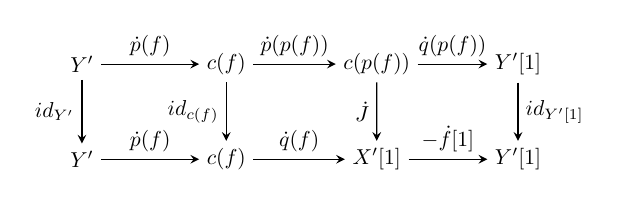
\begin{tikzpicture}[>=stealth,scale=0.78,every node/.style={transform shape}]
    \node (Y1)  at (0,1.55) {$Y'$};
    \node (Cf1) at (2.35,1.55) {$c(f)$};
    \node (Cpf) at (4.80,1.55) {$c(p(f))$};
    \node (Ys1) at (7.10,1.55) {$Y'[1]$};
    \node (Y2)  at (0,0) {$Y'$};
    \node (Cf2) at (2.35,0) {$c(f)$};
    \node (Xs)  at (4.80,0) {$X'[1]$};
    \node (Ys2) at (7.10,0) {$Y'[1]$};
    \draw[->] (Y1) -- node[above] {$\dot p(f)$} (Cf1);
    \draw[->] (Cf1) -- node[above] {$\dot p(p(f))$} (Cpf);
    \draw[->] (Cpf) -- node[above] {$\dot q(p(f))$} (Ys1);
    \draw[->] (Y2) -- node[above] {$\dot p(f)$} (Cf2);
    \draw[->] (Cf2) -- node[above] {$\dot q(f)$} (Xs);
    \draw[->] (Xs) -- node[above] {$-\dot f[1]$} (Ys2);
    \draw[->] (Y1) -- node[left] {$\operatorname{id}_{Y'}$} (Y2);
    \draw[->] (Cf1) -- node[left] {$\operatorname{id}_{c(f)}$} (Cf2);
    \draw[->] (Cpf) -- node[left] {$\dot J$} (Xs);
    \draw[->] (Ys1) -- node[right] {$\operatorname{id}_{Y'[1]}$} (Ys2);
  \end{tikzpicture}
\end{center}

\VerdierSemanticAnchor{ch1-3-3-3-forward-conclusion}
是 $K(C)$ 中三角的一个同构。

\VerdierSemanticAnchor{ch1-3-3-3-proof-reverse}
现在设三角
$Y\xrightarrow{v}Z\xrightarrow{w}X[1]\xrightarrow{-u[1]}Y[1]$
是特异三角。由 (3.2.4) 可知三角

\VerdierSemanticAnchor{ch1-3-3-3-shifted-triangle}
\begin{equation*}
  Y[-1]\xrightarrow{v[-1]}Z[-1]\xrightarrow{w[-1]}X
  \xrightarrow{u}Y
\end{equation*}
是特异三角，并且，
\VerdierSemanticAnchor{ch1-3-3-3-double-rotation}
将前述论证应用两次，可知三角
\begin{equation*}
  X\xrightarrow{u}Y\xrightarrow{v}Z\xrightarrow{w}X[1]
\end{equation*}
\VerdierSemanticAnchor{ch1-3-3-3-conclusion}
是特异三角，证明完毕。
\endgroup
